\begin{activity} \label{A:1.7.3} 
In this activity, we explore two different functions and classify the points at which each is not differentiable.  Let $g$ be the function given by the rule $g(x) = |x|$, and let $f$ be the function that we have previously explored in Preview Activity~\ref{PA:1.7}, whose graph is given again in Figure~\ref{F:1.7.Act3}.
\ba
	\item Reasoning visually, explain why $g$ is differentiable at every point $x$ such that $x \ne 0$.
	\item Use the limit definition of the derivative to show that $g'(0) = \lim_{h \to 0} \frac{|h|}{h}.$
	\item Explain why $g'(0)$ fails to exist by using small positive and negative values of $h$.
\begin{figure}[h]
\begin{center}
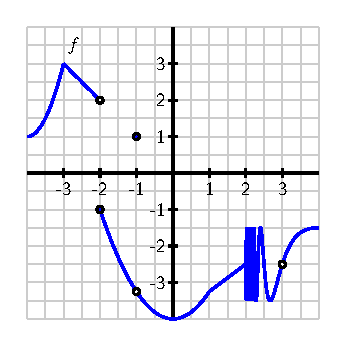
\includegraphics{figures/1_7_PA1.eps}
\caption{The graph of $y = f(x)$ for Activity~\ref{A:1.7.3}.} \label{F:1.7.Act3}
\end{center}
\end{figure}
	\item State all values of $a$ for which $f$ is not differentiable at $x = a$.  For each, provide a reason for your conclusion.
	\item True or false: if a function $p$ is differentiable at $x = b$, then $\lim_{x \to b} p(x)$ must exist.  Why?	
\ea

\end{activity}
\begin{smallhint}
\ba
	\item What type of function is $g$ for all $x < 0$?  For all $x > 0$?
	\item Recall that $g'(0) = \lim_{h \to 0} \frac{g(0 + h) - g(0)}{h}.$
	\item What is the value of $|h|$ when $h < 0$?
	\item You might start by identifying points where $f$ is not continuous.
	\item What does being differentiable at a point tell you about continuity there?	
\ea
\end{smallhint}
\begin{bighint}
\ba
	\item Think about how $g$ is a piecewise linear function.
	\item Recall that $g'(0) = \lim_{h \to 0} \frac{g(0 + h) - g(0)}{h}.$
	\item What is the value of $|h|$ when $h < 0$?  What does this tell you about $\frac{|h|}{h}$ when $h < 0$?
	\item Start by identifying points where $f$ is not continuous.  Then strive to identify any corner points.
	\item What does being differentiable at a point tell you about continuity at that point?	
\ea
\end{bighint}
\begin{activitySolution}
\ba
	\item We know that $g(x) = |x|$ is given by the formula $g(x) = -x$ when $x < 0$ and by $g(x) = x$ when $x \ge 0$.  Each of these pieces of $g$ is a straight line, so at every point other than the point where they meet, the function $g$ has a well-defined slope, and thus is differentiable. 
	\item Observe that
	\begin{eqnarray*}
		g'(0) & = & \lim_{h \to 0} \frac{g(0+h)-g(0)}{h} \\
			& = & \lim_{h \to 0} \frac{|0+h|-|0|}{h} \\
			& = & \lim_{h \to 0} \frac{|h|}{h}
	\end{eqnarray*}
	\item Following up on our work in (b), note that whenever $h > 0$, $|h| = h$, and thus
	$$\lim_{h \to 0^+} \frac{|h|}{h} = \lim_{h \to 0^+} \frac{h}{h} = 1,$$
	while whenever $h < 0$, $|h| = -h$, and thus
	$$\lim_{h \to 0^-} \frac{|h|}{h} = \lim_{h \to 0^-} \frac{-h}{h} = -1$$
	Since the right- and left-hand limits are not equal, it follows that 
	$$g'(0) =  \lim_{h \to 0} \frac{|h|}{h}$$
	does not exist.

	\item $f$ is not differentiable at $a = -2, -1, 2, 3$ because at each of these points $f$ is not continuous.  In addition, $f$ is not differentiable at $a = -3$ and $a = 1$ because the graph of $f$ has a corner point (or cusp) at each of these values.  
	\item True: if a function $p$ is differentiable at $x = b$, then $\lim_{x \to b} p(x)$ must exist.  This is true because we know that if $p$ is differentiable at a point, then $p$ is continuous there, and anytime a function is continuous at a point, it must have a limit there.	
\ea
\end{activitySolution}
\aftera